\section{Phase-Locked Loop}

A Phase-Locked Loop (PLL) is a fundamental electronic circuit used in various communication and signal processing applications.
It operates by synchronizing the frequency of a Voltage-Controlled Oscillator (VCO) with that of an input signal.
The key components of a PLL include a phase detector, a low-pass filter, and the VCO, all connected in a feedback loop. 
The primary function of the PLL is to keep the VCO frequency "locked" to the frequency of the input signal, ensuring they remain in sync.
\begin{figure}[H]
    \centering
    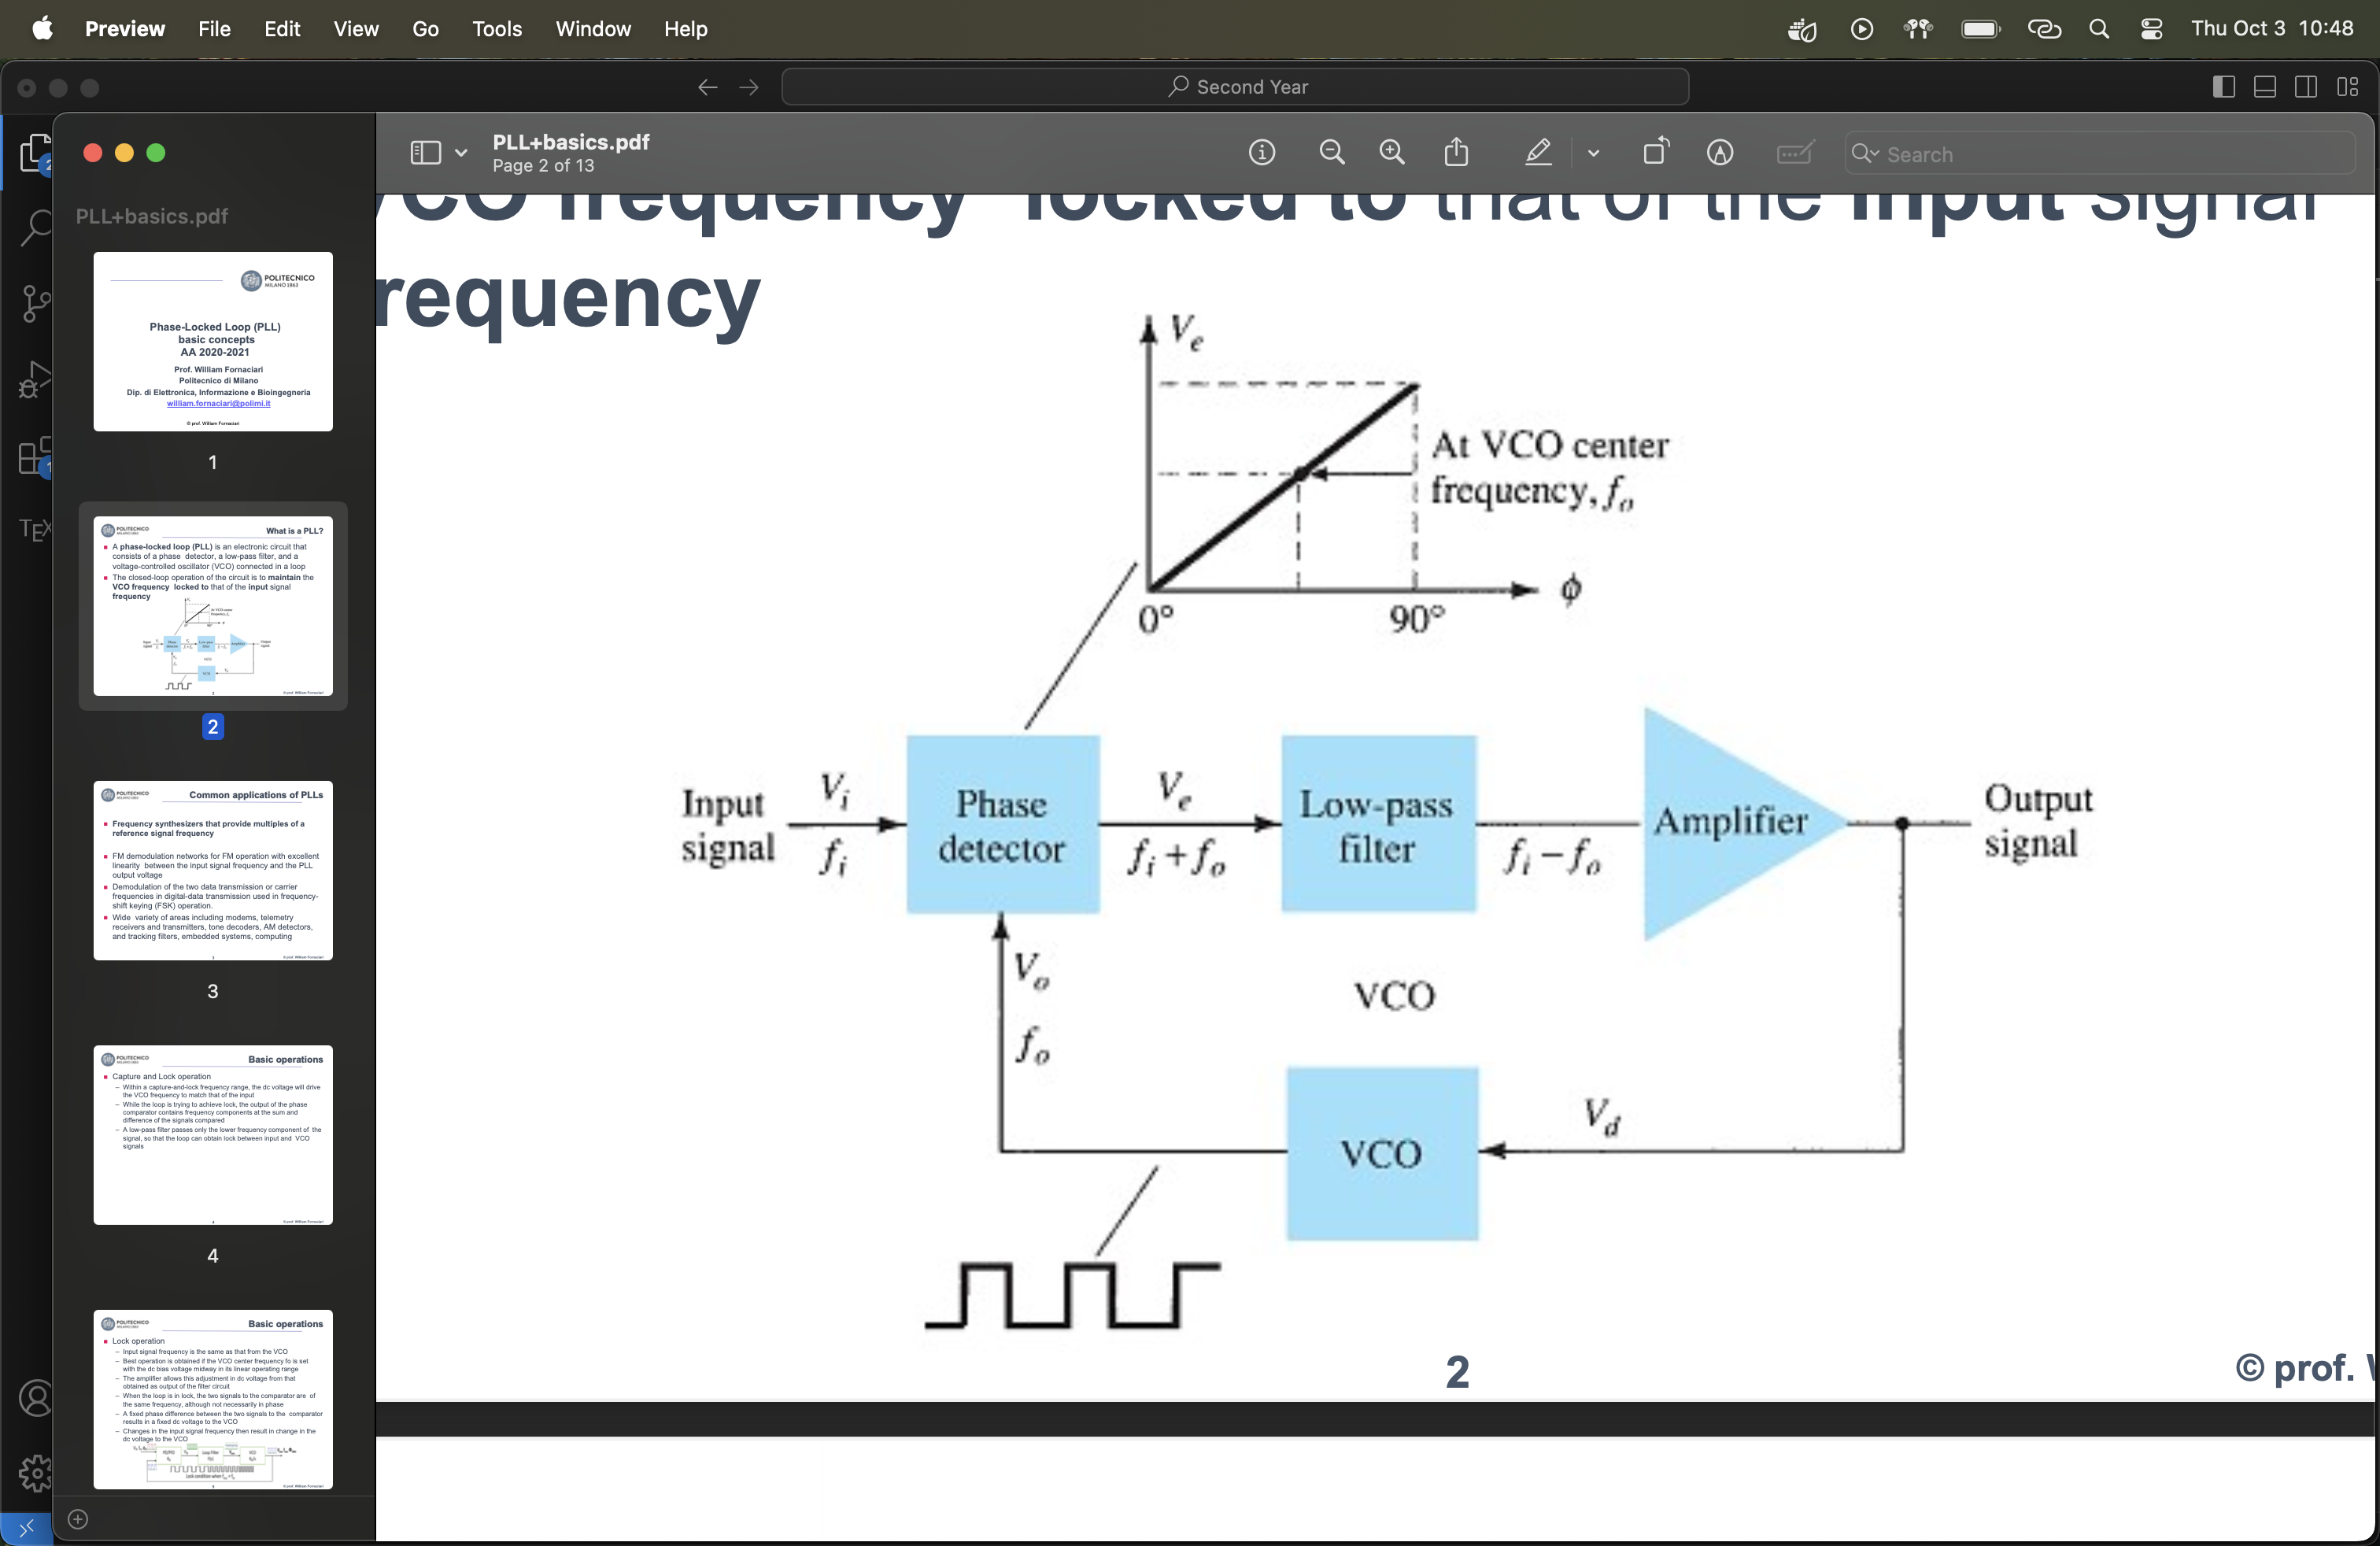
\includegraphics[width=0.75\linewidth]{images/pll.png}
    \caption{Phase-Locked Lopp}
\end{figure}

\subsection{Locking mechanism}
The fundamental goal of the PLL is to align the VCO's output frequency with the input signal frequency. 
The best performance is achieved when the VCO's center frequency, $f_{{o}}$, is set within the middle of its linear range using a DC bias voltage.
This allows the circuit to maintain control over the VCO's frequency with maximum efficiency.

In normal operation, when the loop is locked, the input and VCO output frequencies are identical. 
However, they may not necessarily be in phase. 
The phase detector generates a fixed phase difference between these signals, which is converted into a DC control voltage applied to the VCO. 
As the input signal frequency fluctuates, the phase detector adjusts this DC voltage to maintain synchronization.

Due to the limited operating range of the VCO and the feedback nature of the PLL, two key frequency ranges are critical for proper operation:
\begin{itemize}
    \item \textit{Capture range}: the frequency range around the VCO's free-running frequency, $f_{{o}}$, within which the PLL can initially acquire lock with the input signal.
    \item \textit{Lock range}: once the PLL is locked, it can maintain synchronization with the input signal over a wider frequency range than the capture range. 
        This lock range ensures the PLL can handle variations in the input signal while maintaining phase coherence.
\end{itemize}
Phase-Locked Loops (PLLs) are essential components in modern electronics due to their versatile functionality. 
Here are some of the key applications:

\subsection{Applications}
The main applications of a PLL include:
\begin{itemize}
    \item \textit{Clock multiplier or clock generator}: generates a clock signal that is a multiple of the input frequency or provides multiple clock outputs.
    \item \textit{Frequency synthesizer (fractional-N, integer-N)}: produces a clock signal with an arbitrary frequency by dividing or multiplying a reference clock.
    \item \textit{Clock and data recovery}: recovers digital data and a synchronized clock signal from a serial data stream, using a specialized phase detector.
    \item \textit{FM demodulation}: demodulates a radio signal by tracking the frequency modulation and converting it into a usable signal.
\end{itemize}

\paragraph*{Frequency syntesis}
In frequency synthesis applications, a frequency divider is placed between the VCO output and the phase comparator. 
The output frequency, $f_{{o}}$, is divided down before being fed back to the phase detector. 
As long as the loop remains locked, the VCO output will be an integer multiple of the input frequency. 
This principle is widely used in communication systems to generate precise clock signals.
\begin{figure}[H]
    \centering
    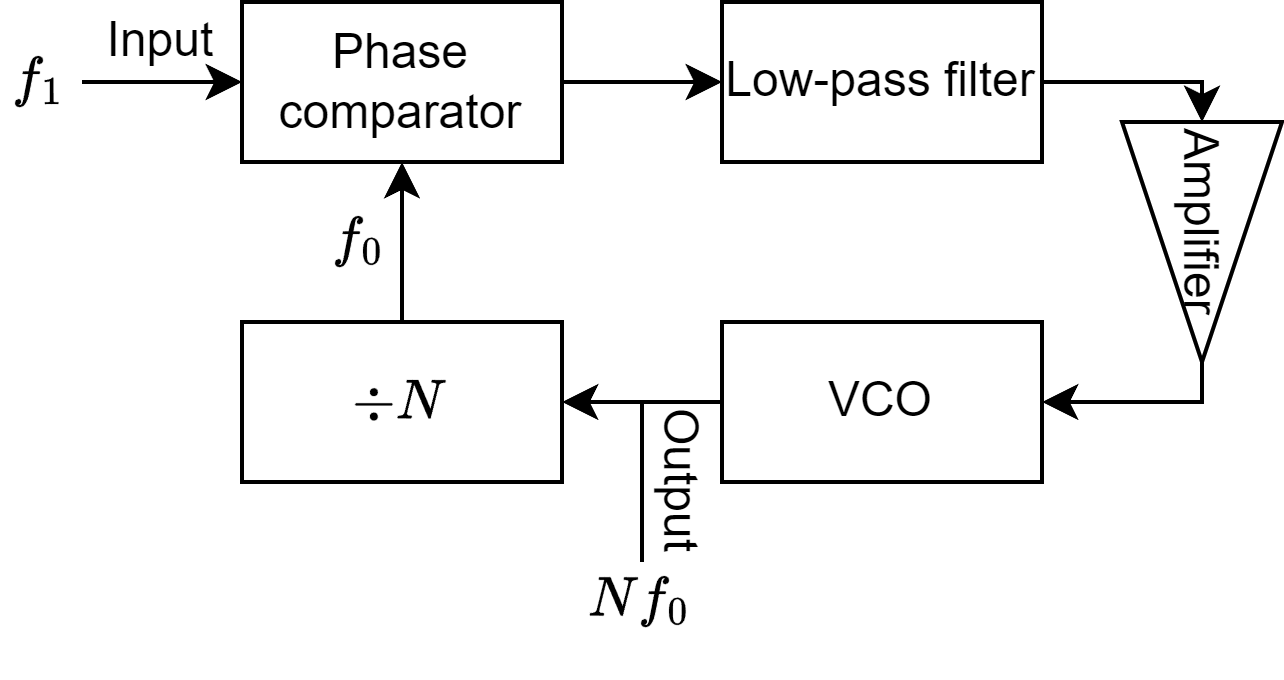
\includegraphics[width=0.65\linewidth]{images/freq.png}
    \caption{Frequency synthesis}
\end{figure}

\paragraph*{Integer-N synthesizer}
The resolution of the output frequency in an Integer-N synthesizer is determined by the reference frequency applied to the phase detector. 
The step size or frequency resolution represents the smallest frequency increment the system can generate. 
This approach simplifies creating low-frequency sources, as producing a stable frequency in the kilohertz (kHz) range directly from a crystal oscillator can be impractical due to its large size.

A more practical solution is to use a stable, high-frequency crystal oscillator and divide its output using an Integer-N synthesizer.
The output frequency $f_{{o}}$ can be expressed as:
\[f_{{o}}=f_{\text{ref}}\dfrac{n}{r}\]
Here, $f_{\text{ref}}$ is the reference frequency (often derived from a crystal oscillator), $n$ and $r$ are programmable integer values that can be selected based on system requirements.

By adjusting $N$ and $R$, the synthesizer can generate multiple clock frequencies from a single crystal oscillator, allowing for efficient clock domain creation and variable-speed operation in computing systems.
\begin{figure}[H]
    \centering
    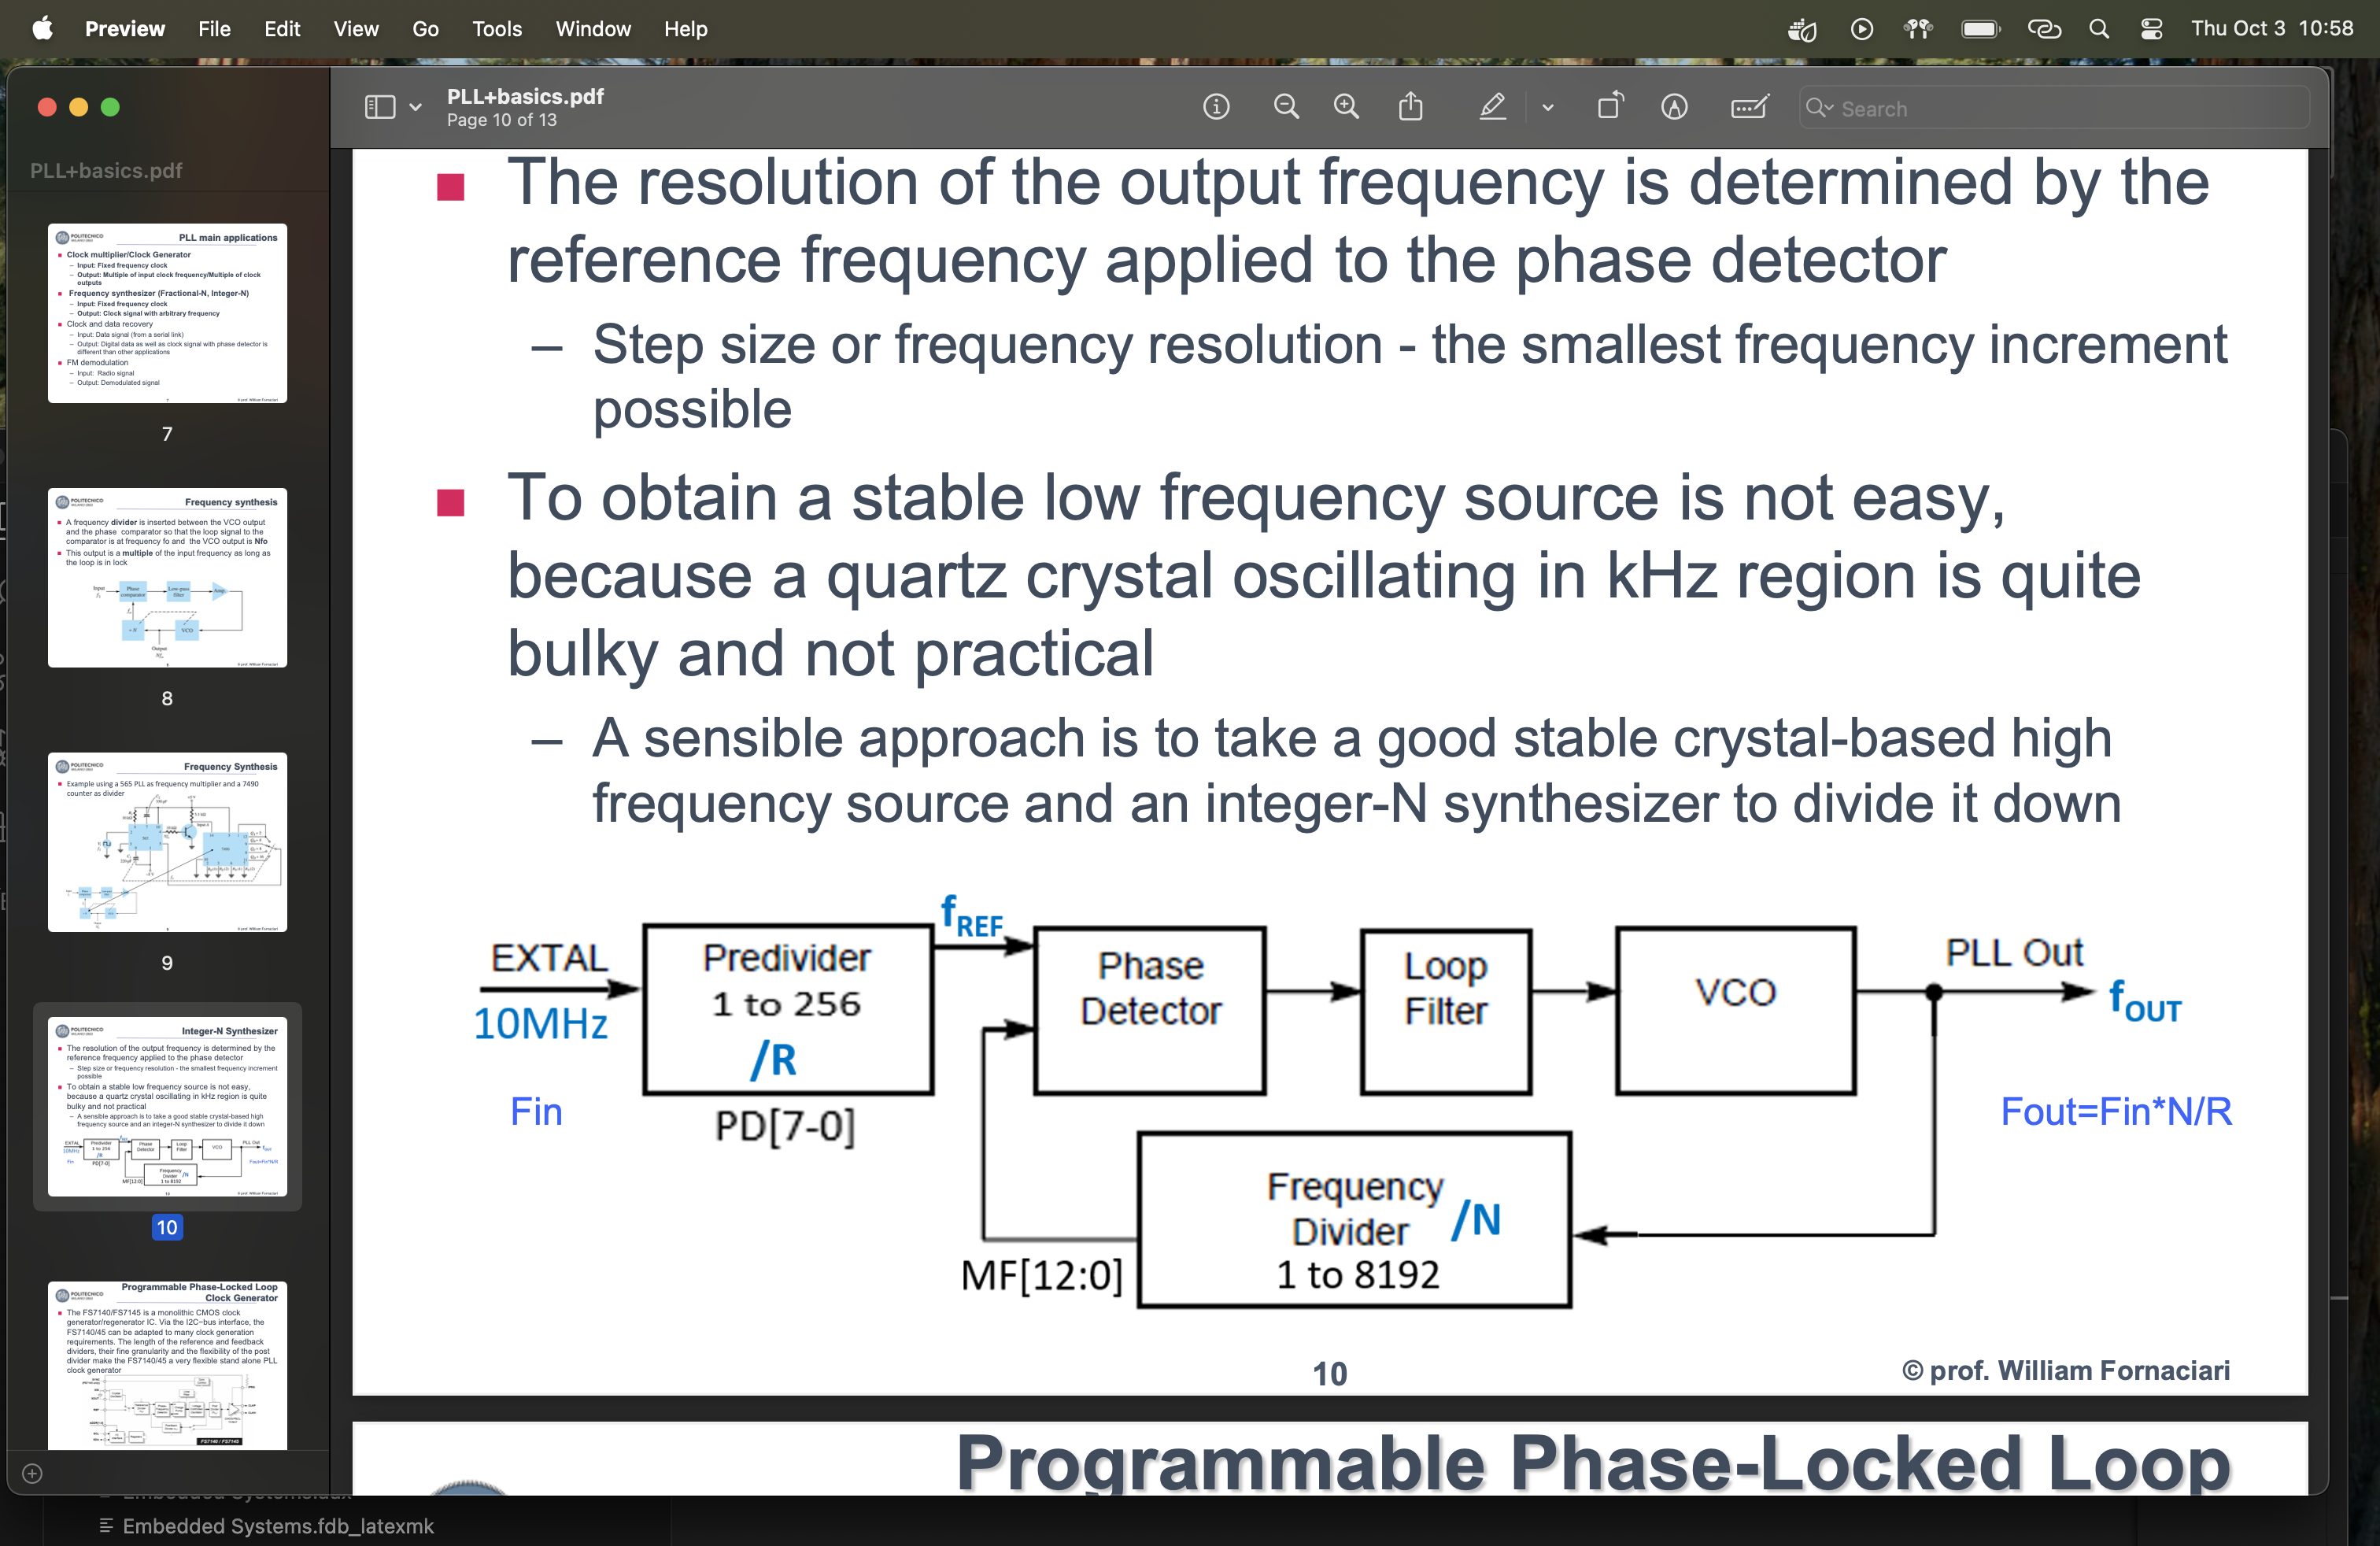
\includegraphics[width=0.75\linewidth]{images/freqn.png}
    \caption{Integer-N synthesis}
\end{figure}

\paragraph*{Integer-N synthesizer with prescalers}
To extend the frequency range of a synthesizer while still allowing low-frequency synthesis, prescalers are introduced. 
Prescalers are frequency dividers that reduce the frequency of the VCO before it reaches the phase detector. 
This technique is essential in systems, such as microcontrollers, where the clock frequency is fixed at design time, but dynamic frequency scaling is needed to save power or manage thermal performance.

A four-modulus prescaler is a logical extension of the traditional dual-modulus prescaler, offering more flexibility. 
It provides four scaling factors and uses two control signals to select one of the available factors. 
This allows the synthesizer to operate over a wider range of frequencies, covering both high and low-frequency requirements.
\begin{figure}[H]
    \centering
    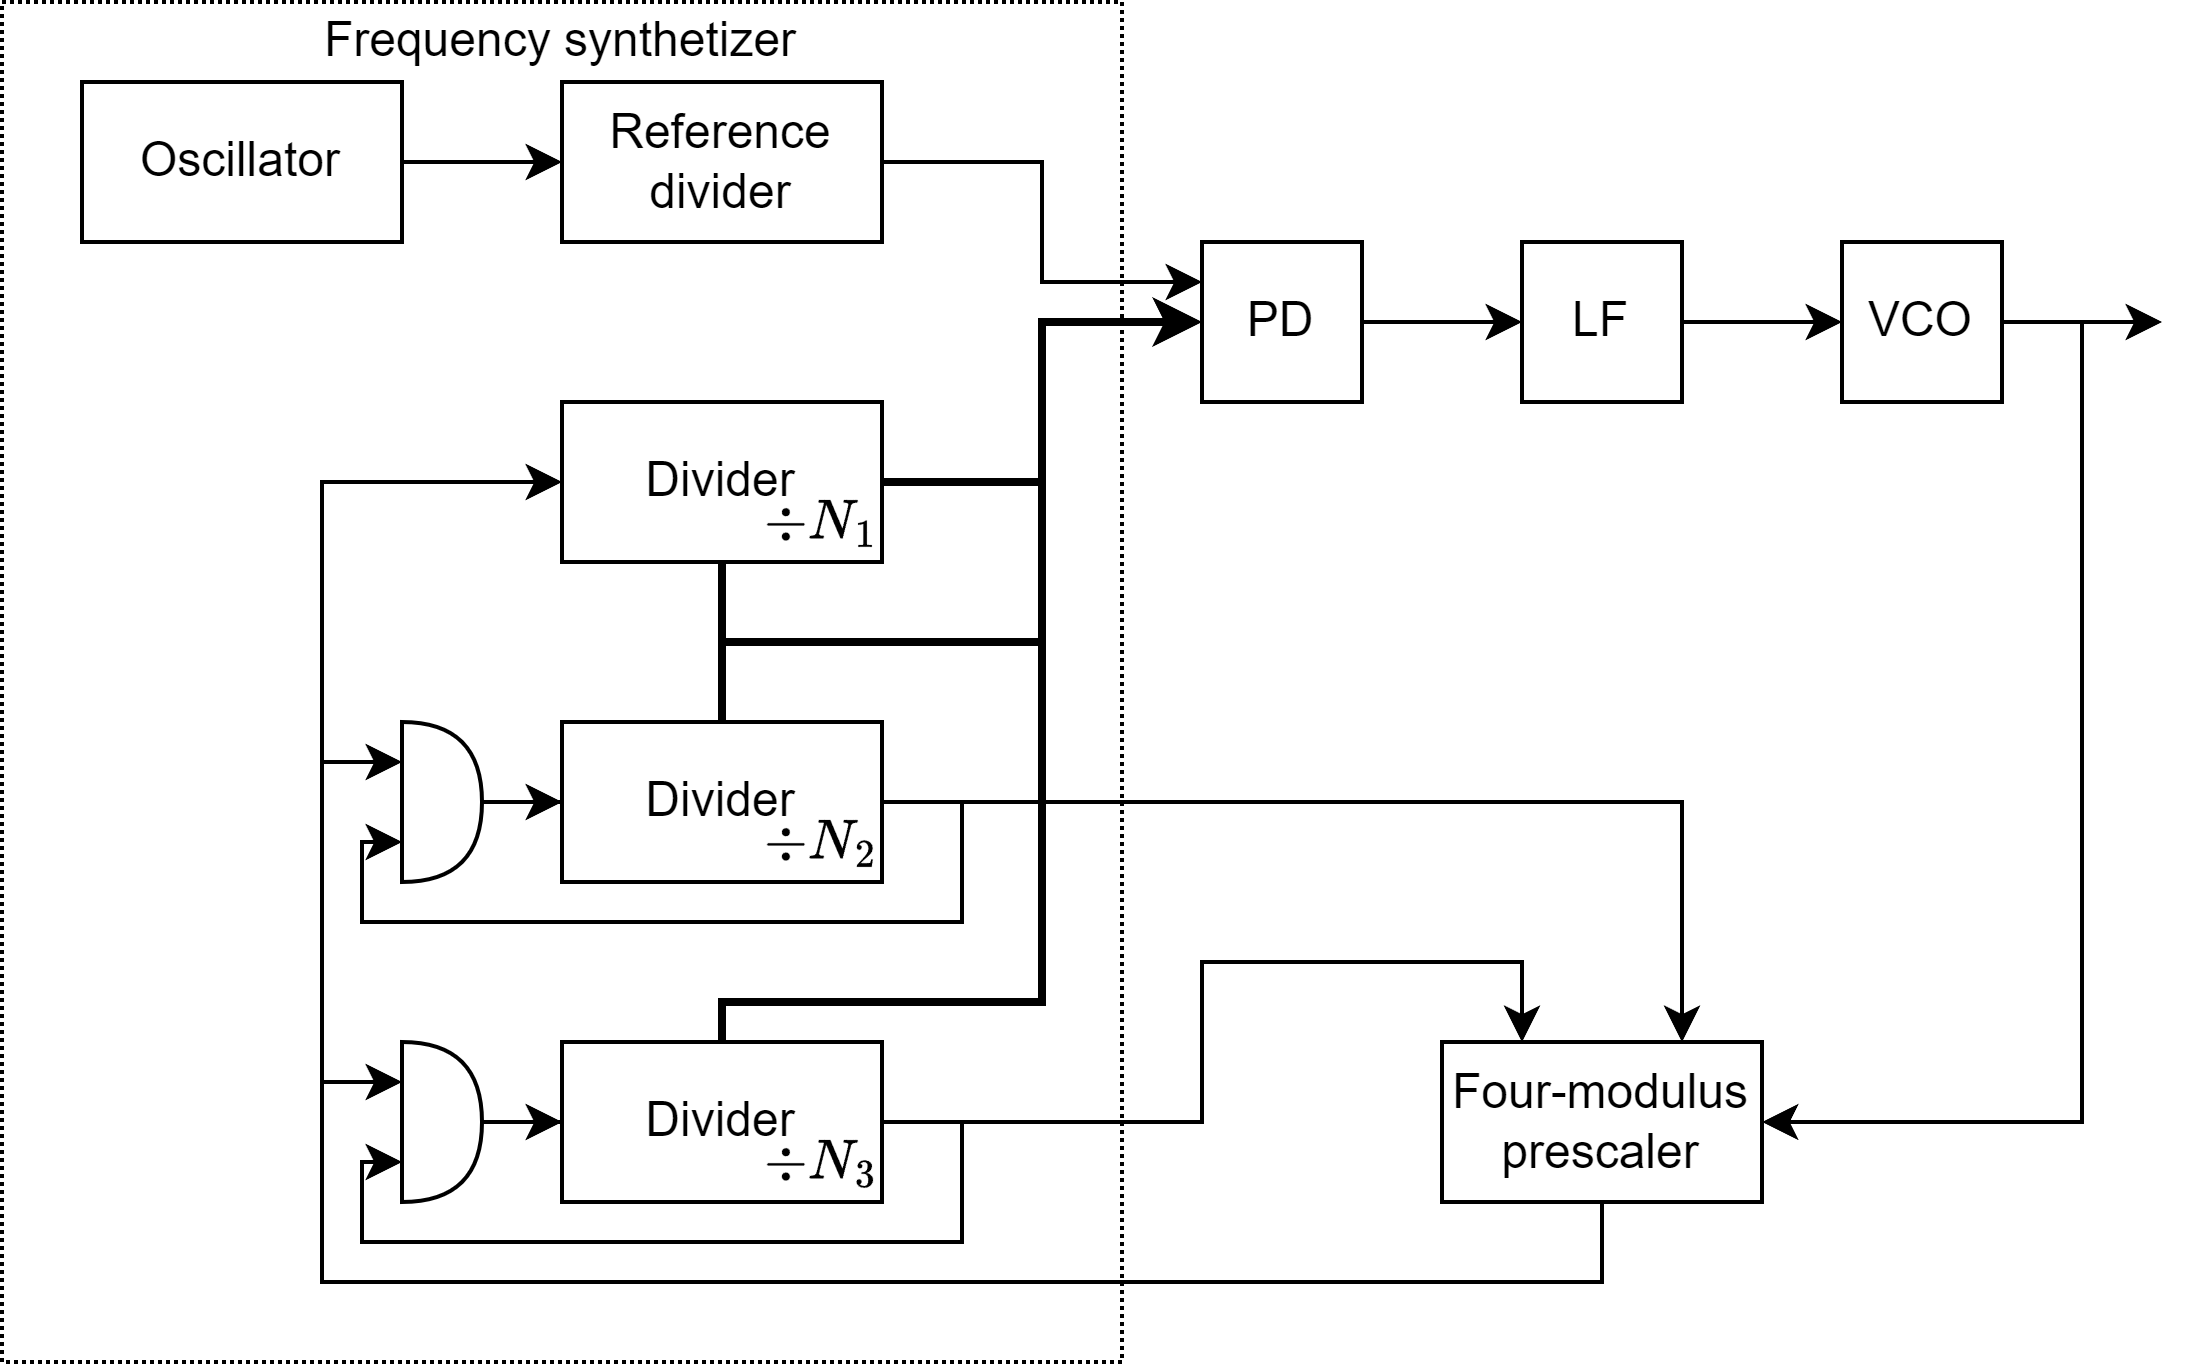
\includegraphics[width=0.75\linewidth]{images/freqp.png}
    \caption{Integer-N synthesis with prescalers}
\end{figure}
In high-end embedded systems, such a design allows dynamic adjustment of clock speeds to optimize performance and power consumption.
By combining prescalers with PLLs, systems can adapt to variable computational loads while maintaining efficient power use.